\documentclass[aspectratio=169,11pt]{beamer}
\usetheme{metropolis}
\usepackage{tikz}
\usetikzlibrary{arrows.meta,positioning,calc}
\usepackage{booktabs}
\usepackage{xcolor}
\usepackage{amsmath}
\usepackage{hyperref}
\usepackage{array}
\newcolumntype{L}[1]{>{\raggedright\arraybackslash}p{#1}}

% === Color palette ===
\definecolor{report}{HTML}{3498DB}
\definecolor{state}{HTML}{9B59B6}
\definecolor{bias}{HTML}{E67E22}
\definecolor{neutral}{HTML}{95A5A6}
\definecolor{pass}{HTML}{27AE60}
\definecolor{fail}{HTML}{E74C3C}
\tikzset{
  box/.style={draw=#1,thick,rounded corners,fill=#1!10,minimum width=3.2cm,minimum height=0.9cm,font=\small,align=center},
  boxL/.style={draw=#1,thick,rounded corners,fill=#1!10,minimum width=5.2cm,minimum height=1.2cm,font=\small,align=center},
  boxS/.style={draw=#1,thick,rounded corners,fill=#1!10,minimum width=2.8cm,minimum height=0.9cm,font=\footnotesize,align=center},
  panel/.style={draw=#1,thick,rounded corners,fill=#1!8},
  arr/.style={-{Stealth},thick,neutral},
  elab/.style={font=\scriptsize,text=black},
  rung/.style={draw=#1,thick,rounded corners,fill=#1!10,minimum width=4.4cm,minimum height=0.75cm,font=\small\bfseries,align=center},
}
\hypersetup{colorlinks=true,linkcolor=.,urlcolor=report}

\title{Philosophy of Introspection}
\subtitle{Which sense of introspection an LLM experiment measures}
\author{Measuring AI Self-Reports}
\date{}

\newcommand{\partslide}[2]{%
\begin{frame}[plain,label=#1]
\vfill
\begin{center}
  \setlength{\fboxrule}{2.5pt}%
  \fcolorbox{black}{white}{\parbox{0.65\textwidth}{\centering\vspace{0.8em}
    {\Large\bfseries #2}
  \vspace{0.8em}}}
\end{center}
\vfill
\end{frame}}

\newcommand{\site}{https://measuring-self-reports.github.io/measuring-self-reports}

\begin{document}

\begin{frame}[plain,noframenumbering]
\vspace*{-0.6cm}\titlepage
\end{frame}

%% --- Overview ---
\begin{frame}{Overview}\footnotesize
\begin{columns}[T]
\begin{column}{0.48\textwidth}
\hyperlink{part1}{\textbf{Part 1: The question}}\\[0.15em]
{\scriptsize%
\quad\hyperlink{hungry}{1.~Knowing your own mind}\\%
\quad\hyperlink{examples}{2.~Two running examples}%
}\vspace{0.3em}

\hyperlink{part2}{\textbf{Part 2: A liberal definition}}\\[0.15em]
{\scriptsize%
\quad\hyperlink{kfdef}{3.~Three conditions}\\%
\quad\hyperlink{kfloose}{4.~How much the definition lets in}\\%
\quad\hyperlink{kfsources}{5.~Three sources of variation in a report}%
}\vspace{0.3em}

\hyperlink{part3}{\textbf{Part 3: A causal criterion}}\\[0.15em]
{\scriptsize%
\quad\hyperlink{causal}{6.~Caused by the state it describes}\\%
\quad\hyperlink{twocases}{7.~Creative process and temperature}\\%
\quad\hyperlink{temp}{8.~The route in the temperature case}%
}
\end{column}
\begin{column}{0.48\textwidth}
\hyperlink{part4}{\textbf{Part 4: Knowing it is you}}\\[0.15em]
{\scriptsize%
\quad\hyperlink{objperc}{9.~Object-perception model}\\%
\quad\hyperlink{reliab}{10.~Reliability account}\\%
\quad\hyperlink{selfspec}{11.~Self-specifying information}\\%
\quad\hyperlink{selfother}{12.~Self-versus-other test}\\%
\quad\hyperlink{further}{13.~Two further objections}%
}\vspace{0.3em}

\hyperlink{part5}{\textbf{Part 5: Four senses}}\\[0.15em]
{\scriptsize%
\quad\hyperlink{ladder}{14.~Four senses, weakest to strongest}\\%
\quad\hyperlink{designs}{15.~One design per sense}\\%
\quad\hyperlink{confound}{16.~A route through public output}\\%
\quad\hyperlink{measmodel}{17.~Mimicry and the measurement model}%
}\vspace{0.3em}

\hyperlink{part6}{\textbf{Part 6: Limits}}\\[0.15em]
{\scriptsize%
\quad\hyperlink{limits}{18.~Where the analogy stops}\\%
\quad\hyperlink{summary}{19.~Summary}\\%
\quad\hyperlink{reading}{20.~Reading}%
}
\end{column}
\end{columns}
\end{frame}

%% ============================================================
\partslide{part1}{Part 1\\[0.5em]{\large\mdseries The question}}
%% ============================================================

\begin{frame}[label=hungry]{Knowing your own mind}
Compare two sentences:

\vspace{0.5em}
\begin{center}
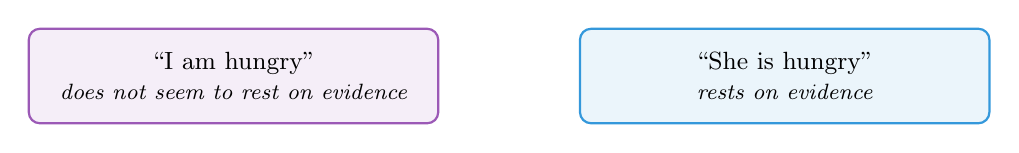
\begin{tikzpicture}
  \node[boxL=state] (me) at (0,0) {``I am hungry''\\{\footnotesize\itshape does not seem to rest on evidence}};
  \node[boxL=report] (her) at (7,0) {``She is hungry''\\{\footnotesize\itshape rests on evidence}};
\end{tikzpicture}
\end{center}

\vspace{0.5em}
Philosophy of introspection asks what makes the first kind of knowledge different from the second. Philosophers disagree about the answer.

\vspace{0.5em}
{\small For a large language model (LLM), the disagreement decides what an experiment measures. Before a paper can say a model introspects, it has to say which sense of introspection its procedure is built to detect. Four philosophical positions give four senses, from weakest to strongest.}
\end{frame}

\begin{frame}[label=examples]{Two running examples}
\begin{columns}[T]
\begin{column}{0.48\textwidth}
\begin{center}
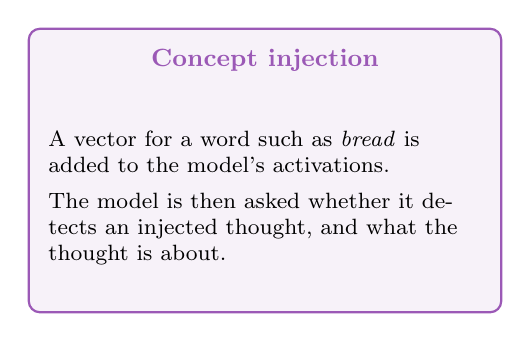
\begin{tikzpicture}
  \draw[panel=state] (0,0) rectangle (6,3.6);
  \node[font=\small\bfseries,state] at (3,3.2) {Concept injection};
  \node[font=\footnotesize,align=left,text width=5.5cm] at (3,1.45) {A vector for a word such as \emph{bread} is added to the model's activations.\\[0.4em]
  The model is then asked whether it detects an injected thought, and what the thought is about.};
\end{tikzpicture}
\end{center}
\end{column}
\begin{column}{0.48\textwidth}
\begin{center}
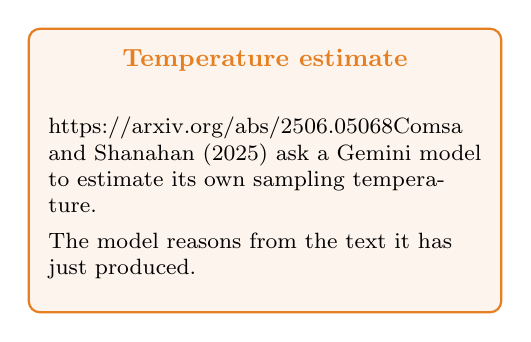
\begin{tikzpicture}
  \draw[panel=bias] (0,0) rectangle (6,3.6);
  \node[font=\small\bfseries,bias] at (3,3.2) {Temperature estimate};
  \node[font=\footnotesize,align=left,text width=5.5cm] at (3,1.45) {\href{https://arxiv.org/abs/2506.05068}{Comsa and Shanahan (2025)} ask a Gemini model to estimate its own sampling temperature.\\[0.4em]
  The model reasons from the text it has just produced.};
\end{tikzpicture}
\end{center}
\end{column}
\end{columns}

\vspace{0.7em}
{\small Both end in a self-report. Each position in this deck asks a different question about how that self-report came about.}
\end{frame}

%% ============================================================
\partslide{part2}{Part 2\\[0.5em]{\large\mdseries A liberal definition}}
%% ============================================================

\begin{frame}[label=kfdef]{Three conditions}
\href{https://philarchive.org/archive/KAMWFC}{Kammerer and Frankish (2023)} want a definition that also covers animals and machines:

\vspace{0.3em}
{\small\itshape ``Introspection is a process by which a cognitive system represents its own current mental states, in a manner that allows the information to be used for online behavioural control.''}

\vspace{0.5em}
\begin{center}
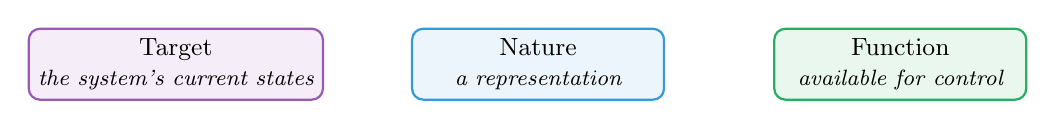
\begin{tikzpicture}
  \node[box=state] (t) at (0,0) {Target\\{\footnotesize\itshape the system's current states}};
  \node[box=report] (n) at (4.6,0) {Nature\\{\footnotesize\itshape a representation}};
  \node[box=pass] (f) at (9.2,0) {Function\\{\footnotesize\itshape available for control}};
\end{tikzpicture}
\end{center}

\vspace{0.4em}
{\small A human version: you notice you are hungry, and that information is there to steer what you do next. An AI version: the definition names artificial systems that monitor their own resources, or whether they have the knowledge a task needs, as candidate cases.}
\end{frame}

\begin{frame}[label=kfloose]{How much the definition lets in}
The definition is permissive on purpose:

\vspace{0.4em}
\begin{itemize}\setlength\itemsep{6pt}
  \item {\small \textbf{States that happen to be mental.} The process must represent a mental state, but need not represent it \emph{as} mental.}
  \item {\small \textbf{Available, not necessarily used.} The information has to be available for control. Nobody has to act on it.}
  \item {\small \textbf{Inference counts.} Interpreting yourself, or applying a theory of mind to yourself, qualifies.}
\end{itemize}

\vspace{0.4em}
\begin{center}

\begin{tikzpicture}
  \draw[panel=fail] (0,0) rectangle (12.4,1.3);
  \node[font=\small\bfseries,fail,anchor=west] at (0.3,0.65) {Excluded};
  \node[font=\footnotesize,align=left,text width=9.8cm,anchor=west] at (2.2,0.65) {A scientist reading their own brain scan. The information is not available for online control, so it is not introspection.};
\end{tikzpicture}
\end{center}
\end{frame}

\begin{frame}[label=kfsources]{Three sources of variation in a report}
When someone says ``I am hungry,'' three different things could make the report vary:

\vspace{0.5em}
\begin{center}
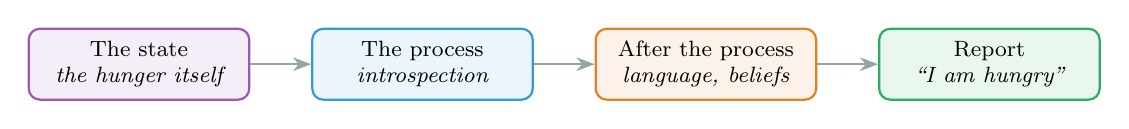
\begin{tikzpicture}
  \node[boxS=state] (s) at (0,0) {The state\\{\footnotesize\itshape the hunger itself}};
  \node[boxS=report] (p) at (3.6,0) {The process\\{\footnotesize\itshape introspection}};
  \node[boxS=bias] (v) at (7.2,0) {After the process\\{\footnotesize\itshape language, beliefs}};
  \node[boxS=pass] (r) at (10.8,0) {Report\\{\footnotesize\itshape ``I am hungry''}};
  \draw[arr] (s) -- (p);
  \draw[arr] (p) -- (v);
  \draw[arr] (v) -- (r);
\end{tikzpicture}
\end{center}

\vspace{0.5em}
Kammerer and Frankish point out that data about responses alone underdetermine which of the three produced a given report.

\vspace{0.4em}
{\small For the bread example: the report ``I detect a thought about bread'' could vary because the internal state varied, because the route from state to report varied, or because of how the model puts things into words.}
\end{frame}

%% ============================================================
\partslide{part3}{Part 3\\[0.5em]{\large\mdseries A causal criterion}}
%% ============================================================

\begin{frame}[label=causal]{Caused by the state it describes}
Comsa and Shanahan adapt a lightweight account to LLMs. A self-report is introspective if:

\vspace{0.2em}
\begin{center}
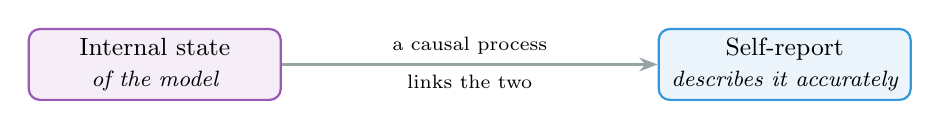
\begin{tikzpicture}
  \node[box=state] (s) at (0,0) {Internal state\\{\footnotesize\itshape of the model}};
  \node[box=report] (r) at (8,0) {Self-report\\{\footnotesize\itshape describes it accurately}};
  \draw[arr] (s) -- node[above,elab]{a causal process} node[below,elab]{links the two} (r);
\end{tikzpicture}
\end{center}

\vspace{0.2em}
\begin{itemize}\setlength\itemsep{2pt}
  \item {\small \textbf{Lightweight:} it drops the requirements that introspection be immediate or involve self-presence.}
  \item {\small \textbf{Internal states, not mental states:} the wording avoids implying that the model is conscious.}
\end{itemize}

{\small A human version: ``I am hungry'' counts if the hunger is what produced the sentence, and not, say, the habit of saying it at noon.}
\end{frame}

\begin{frame}[label=twocases]{Creative process and temperature}
They test the criterion on two cases with Gemini models:

\vspace{0.5em}
\begin{columns}[T]
\begin{column}{0.48\textwidth}
\begin{center}
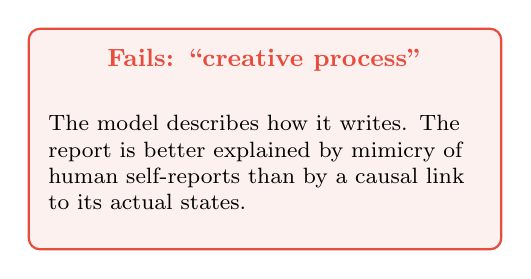
\begin{tikzpicture}
  \draw[panel=fail] (0,0) rectangle (6,2.8);
  \node[font=\small\bfseries,fail] at (3,2.4) {Fails: ``creative process''};
  \node[font=\footnotesize,align=left,text width=5.5cm] at (3,1.1) {The model describes how it writes. The report is better explained by mimicry of human self-reports than by a causal link to its actual states.};
\end{tikzpicture}
\end{center}
\end{column}
\begin{column}{0.48\textwidth}
\begin{center}
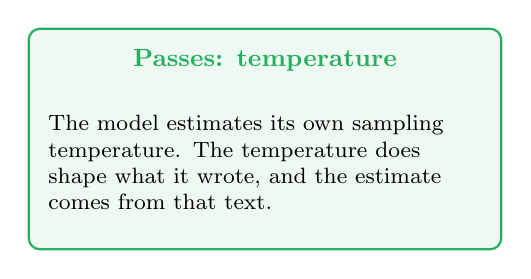
\begin{tikzpicture}
  \draw[panel=pass] (0,0) rectangle (6,2.8);
  \node[font=\small\bfseries,pass] at (3,2.4) {Passes: temperature};
  \node[font=\footnotesize,align=left,text width=5.5cm] at (3,1.1) {The model estimates its own sampling temperature. The temperature does shape what it wrote, and the estimate comes from that text.};
\end{tikzpicture}
\end{center}
\end{column}
\end{columns}

\vspace{0.7em}
{\small The two cases are illustrations of the criterion, not a study of how accurate the model is.}
\end{frame}

\begin{frame}[label=temp]{The route in the temperature case}
A human version: you guess how tired you were last night by rereading the messages you sent.

\vspace{0.5em}
\begin{center}
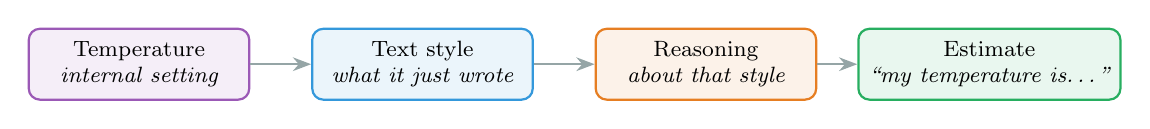
\begin{tikzpicture}
  \node[boxS=state] (t) at (0,0) {Temperature\\{\footnotesize\itshape internal setting}};
  \node[boxS=report] (x) at (3.6,0) {Text style\\{\footnotesize\itshape what it just wrote}};
  \node[boxS=bias] (r) at (7.2,0) {Reasoning\\{\footnotesize\itshape about that style}};
  \node[boxS=pass] (e) at (10.8,0) {Estimate\\{\footnotesize\itshape ``my temperature is\dots''}};
  \draw[arr] (t) -- (x);
  \draw[arr] (x) -- (r);
  \draw[arr] (r) -- (e);
\end{tikzpicture}
\end{center}

\vspace{0.6em}
Every arrow is causal, so the report meets the causal criterion.

\vspace{0.3em}
{\small The second box is the text the model produced. Part~4 asks whether it matters that this text is public.}
\end{frame}

%% ============================================================
\partslide{part4}{Part 4\\[0.5em]{\large\mdseries Knowing it is you}}
%% ============================================================

\begin{frame}[label=objperc]{Object-perception model}
\href{https://philpapers.org/rec/SHOSAI-2}{Shoemaker (1994)} asks whether self-knowledge works like perception.

\vspace{0.4em}
\begin{columns}[T]
\begin{column}{0.48\textwidth}
\begin{center}
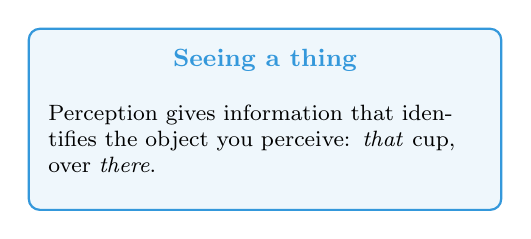
\begin{tikzpicture}
  \draw[panel=report] (0,0) rectangle (6,2.3);
  \node[font=\small\bfseries,report] at (3,1.9) {Seeing a thing};
  \node[font=\footnotesize,align=left,text width=5.5cm] at (3,0.9) {Perception gives information that identifies the object you perceive: \emph{that} cup, over \emph{there}.};
\end{tikzpicture}
\end{center}
\end{column}
\begin{column}{0.48\textwidth}
\begin{center}
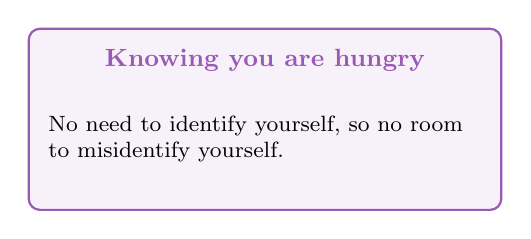
\begin{tikzpicture}
  \draw[panel=state] (0,0) rectangle (6,2.3);
  \node[font=\small\bfseries,state] at (3,1.9) {Knowing you are hungry};
  \node[font=\footnotesize,align=left,text width=5.5cm] at (3,0.9) {No need to identify yourself, so no room to misidentify yourself.};
\end{tikzpicture}
\end{center}
\end{column}
\end{columns}

\vspace{0.6em}
{\small\itshape ``if I have my usual access to my hunger, there is no room for the thought `Someone is hungry all right, but is it me?'\,''}

\vspace{0.4em}
{\small This property is called \textbf{immunity to error through misidentification} (IEM).}
\end{frame}

\begin{frame}[label=reliab]{Reliability account}
Shoemaker's alternative to the perception model:

\vspace{0.6em}
\begin{center}
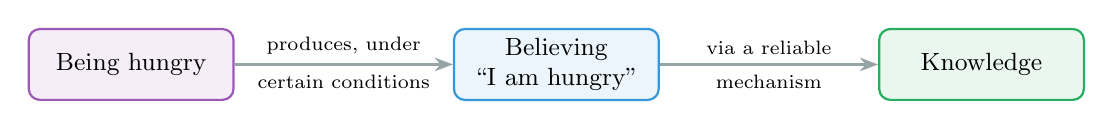
\begin{tikzpicture}
  \node[box=state,minimum width=2.6cm] (s) at (0,0) {Being hungry};
  \node[box=report,minimum width=2.6cm] (b) at (5.4,0) {Believing\\``I am hungry''};
  \node[box=pass,minimum width=2.6cm] (k) at (10.8,0) {Knowledge};
  \draw[arr] (s) -- node[above,elab]{produces, under} node[below,elab]{certain conditions} (b);
  \draw[arr] (b) -- node[above,elab]{via a reliable} node[below,elab]{mechanism} (k);
\end{tikzpicture}
\end{center}

\vspace{0.6em}
The belief counts as knowledge because the mechanism that produced it is reliable, not because of any evidence behind it.

\vspace{0.4em}
{\small On this account the question for an experiment is about the mechanism that links a state to the belief about it.}
\end{frame}

\begin{frame}[label=selfspec]{Self-specifying information}
\href{https://philarchive.org/rec/ZAKMTS}{Zakharova (2025)} grants Comsa and Shanahan their causal link, then asks whether the judgment is about the self in the right way.

\vspace{0.4em}
{\small IEM needs \textbf{self-specifying} information: information that leaves no room to misidentify who is in the state.}

\vspace{0.2em}
\begin{center}
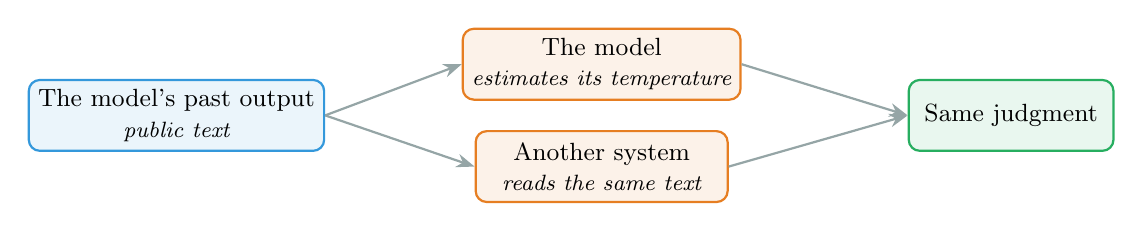
\begin{tikzpicture}
  \node[box=report] (x) at (0,0) {The model's past output\\{\footnotesize\itshape public text}};
  \node[box=bias] (m) at (5.4,0.65) {The model\\{\footnotesize\itshape estimates its temperature}};
  \node[box=bias] (o) at (5.4,-0.65) {Another system\\{\footnotesize\itshape reads the same text}};
  \node[box=pass,minimum width=2.6cm] (j) at (10.6,0) {Same judgment};
  \draw[arr] (x.east) -- (m.west);
  \draw[arr] (x.east) -- (o.west);
  \draw[arr] (m.east) -- (j.west);
  \draw[arr] (o.east) -- (j.west);
\end{tikzpicture}
\end{center}

{\small The temperature case fails this test. The model reasons from text anyone can read, so another system could reach the same judgment from it.}
\end{frame}

\begin{frame}[label=selfother]{Self-versus-other test}
A human version: does your guess about how tired you were beat a friend's guess from the same messages?

\vspace{0.5em}
\begin{center}
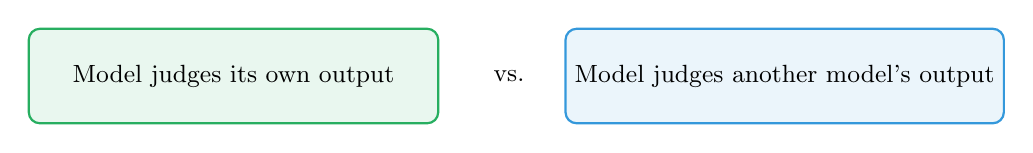
\begin{tikzpicture}
  \node[boxL=pass] (a) at (0,0) {Model judges its own output};
  \node[boxL=report] (b) at (7,0) {Model judges another model's output};
  \node[font=\small,text=black] at (3.5,0) {vs.};
\end{tikzpicture}
\end{center}

\vspace{0.5em}
Zakharova proposes this experiment: test whether models judge their own output better than other models' output.

\vspace{0.4em}
{\small \href{https://arxiv.org/abs/2410.13787}{Binder et al.}\ run a comparison of this kind. A model introspects if it predicts its own behavior better than a second model that was trained on the first model's behavior.}
\end{frame}

\begin{frame}[label=further]{Two further objections}
Zakharova raises two more:

\vspace{0.6em}
\begin{columns}[T]
\begin{column}{0.48\textwidth}
\begin{center}
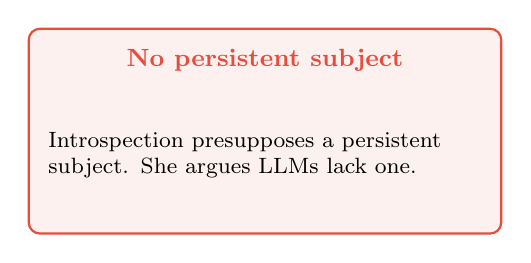
\begin{tikzpicture}
  \draw[panel=fail] (0,0) rectangle (6,2.6);
  \node[font=\small\bfseries,fail] at (3,2.2) {No persistent subject};
  \node[font=\footnotesize,align=left,text width=5.5cm] at (3,1.0) {Introspection presupposes a persistent subject. She argues LLMs lack one.};
\end{tikzpicture}
\end{center}
\end{column}
\begin{column}{0.48\textwidth}
\begin{center}
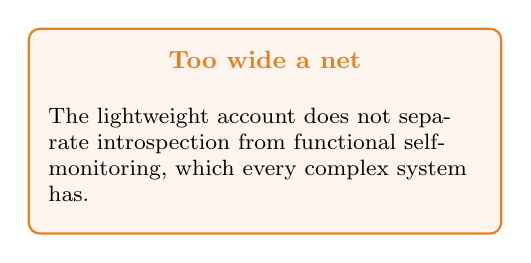
\begin{tikzpicture}
  \draw[panel=bias] (0,0) rectangle (6,2.6);
  \node[font=\small\bfseries,bias] at (3,2.2) {Too wide a net};
  \node[font=\footnotesize,align=left,text width=5.5cm] at (3,1.0) {The lightweight account does not separate introspection from functional self-monitoring, which every complex system has.};
\end{tikzpicture}
\end{center}
\end{column}
\end{columns}

\vspace{0.7em}
{\small The second objection gives a name, \emph{functional self-monitoring}, to the weakest of the four senses in the next part.}
\end{frame}

%% ============================================================
\partslide{part5}{Part 5\\[0.5em]{\large\mdseries Four senses of introspection}}
%% ============================================================

\begin{frame}[label=ladder]{Four senses, weakest to strongest}
\begin{center}
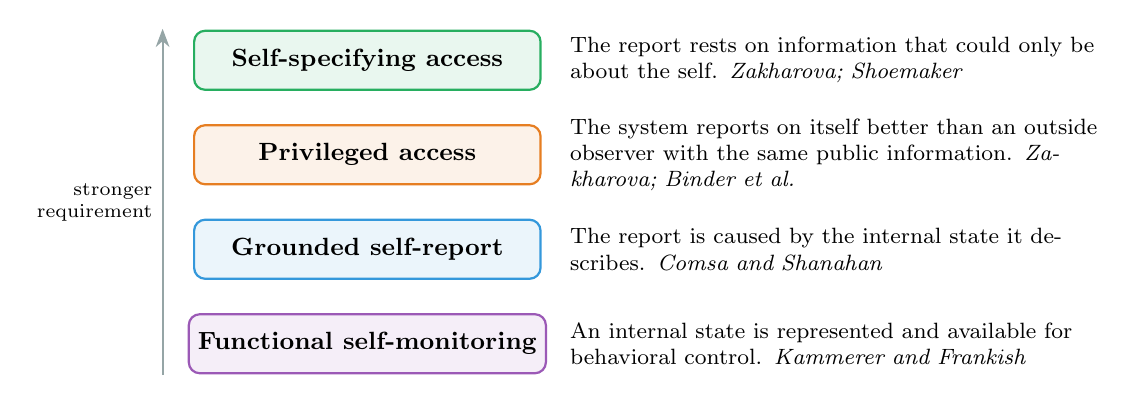
\begin{tikzpicture}
  \node[rung=pass] (d) at (0,3.6) {Self-specifying access};
  \node[rung=bias] (c) at (0,2.4) {Privileged access};
  \node[rung=report] (b) at (0,1.2) {Grounded self-report};
  \node[rung=state] (a) at (0,0) {Functional self-monitoring};
  \draw[arr] (-2.6,-0.4) -- node[left,elab,align=right]{stronger\\requirement} (-2.6,4.0);
  \node[font=\footnotesize,align=left,text width=6.8cm,anchor=west] at (2.45,3.6) {The report rests on information that could only be about the self. \emph{Zakharova; Shoemaker}};
  \node[font=\footnotesize,align=left,text width=6.8cm,anchor=west] at (2.45,2.4) {The system reports on itself better than an outside observer with the same public information. \emph{Zakharova; Binder et al.}};
  \node[font=\footnotesize,align=left,text width=6.8cm,anchor=west] at (2.45,1.2) {The report is caused by the internal state it describes. \emph{Comsa and Shanahan}};
  \node[font=\footnotesize,align=left,text width=6.8cm,anchor=west] at (2.45,0) {An internal state is represented and available for behavioral control. \emph{Kammerer and Frankish}};
\end{tikzpicture}
\end{center}

{\small Concept injection is built to test the second sense. The temperature case meets the second sense and, on Zakharova's reading, fails the fourth.}
\end{frame}

\begin{frame}[label=designs]{One design per sense}
Each sense calls for a different experiment:

\vspace{0.5em}
\begin{center}
{\small\renewcommand{\arraystretch}{1.25}
\begin{tabular}{L{3.2cm}L{9.2cm}}
\toprule
\textbf{Sense} & \textbf{Design} \\
\midrule
\textcolor{report}{\textbf{Grounded self-report}} & Intervene on the internal state and check that the report follows. Concept injection is this design: inject \emph{bread}, see whether the report says bread. \\
\textcolor{bias}{\textbf{Privileged access}} & Compare the model's report about itself with another system's report from the same evidence, as Binder et al.\ do. \\
\textcolor{pass}{\textbf{Self-specifying access}} & Show that the information reaching the report could not have supported a report about another system. \\
\bottomrule
\end{tabular}
}
\end{center}
\end{frame}

\begin{frame}[label=confound]{A route through public output}
Zakharova's objection names a confound for the injection design:

\vspace{0.5em}
\begin{center}
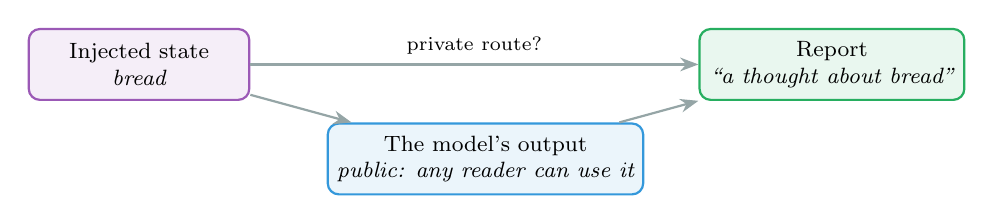
\begin{tikzpicture}
  \node[boxS=state] (i) at (0,0) {Injected state\\{\footnotesize\itshape bread}};
  \node[boxS=report] (o) at (4.4,-1.2) {The model's output\\{\footnotesize\itshape public: any reader can use it}};
  \node[boxS=pass] (r) at (8.8,0) {Report\\{\footnotesize\itshape ``a thought about bread''}};
  \draw[arr] (i) -- node[above,elab]{private route?} (r);
  \draw[arr] (i) -- (o);
  \draw[arr] (o) -- (r);
\end{tikzpicture}
\end{center}

\vspace{0.5em}
The internal state can cause the report by way of the model's own output, and any reader of that output could use it too.

\vspace{0.3em}
{\small A causal link without control over what information reaches the reporter shows grounded self-report. It does not show privileged access.}
\end{frame}

\begin{frame}[label=measmodel]{Mimicry and the measurement model}
\begin{columns}[T]
\begin{column}{0.48\textwidth}
{\small\textbf{Mimicry}}\\[0.3em]
{\footnotesize Comsa and Shanahan's mimicry is an alternative explanation of the indication. In measurement terms it is a \textbf{systematic effect}. It is larger when the elicited report resembles human self-reports in the training data.}

\vspace{0.4em}
{\footnotesize Mimicry is the reason the creative-process report fails the causal criterion.}
\end{column}
\begin{column}{0.48\textwidth}
{\small\textbf{Three terms to separate}}\\[0.3em]
{\footnotesize Kammerer and Frankish's three sources of variation map onto what a measurement model of a self-report has to separate:}

\vspace{0.3em}
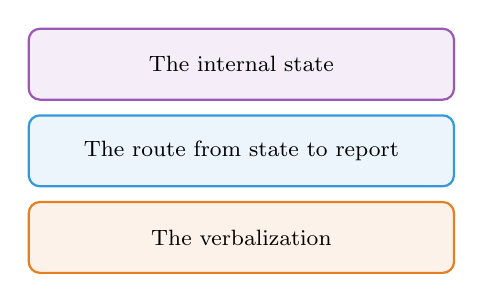
\begin{tikzpicture}
  \node[boxS=state,minimum width=5.4cm] (a) at (0,0) {The internal state};
  \node[boxS=report,minimum width=5.4cm] (b) at (0,-1.1) {The route from state to report};
  \node[boxS=bias,minimum width=5.4cm] (c) at (0,-2.2) {The verbalization};
\end{tikzpicture}
\end{column}
\end{columns}
\end{frame}

%% ============================================================
\partslide{part6}{Part 6\\[0.5em]{\large\mdseries Limits}}
%% ============================================================

\begin{frame}[label=limits]{Where the analogy stops}
\begin{itemize}\setlength\itemsep{10pt}
  \item {\small \textbf{Conceptual, not empirical.} These positions fix what a measurand would be. They supply no instrument, standard or uncertainty. The other foundations on the \href{\site/}{site} supply those.}
  \item {\small \textbf{The measurand may not exist.} If Zakharova is right that current models lack a persistent subject, no procedure measures introspection in her sense. The question for a paper then becomes which weaker sense it measured.}
  \item {\small \textbf{A reply on terms.} Kammerer and Frankish anticipate this objection. They answer that the term can be relabeled rather than abandoned.}
\end{itemize}
\end{frame}

\begin{frame}[label=summary]{Summary}
\begin{center}
{\footnotesize\renewcommand{\arraystretch}{1.15}
\begin{tabular}{L{3.0cm}L{6.3cm}L{3.3cm}}
\toprule
\textbf{Sense} & \textbf{Requirement} & \textbf{Source} \\
\midrule
Functional self-monitoring & A state is represented and available for behavioral control & Kammerer and Frankish; Zakharova \\
Grounded self-report & The report is caused by the state it describes & Comsa and Shanahan \\
Privileged access & Better on itself than an outside observer with the same public information & Zakharova; Binder et al. \\
Self-specifying access & The report rests on information that could not be about another system & Zakharova; Shoemaker \\
\bottomrule
\end{tabular}
}
\end{center}

\vspace{0.2em}
{\footnotesize The \href{\site/measurement-card/measurand/}{measurand} stage of the measurement card asks which of the four a paper tests. Mimicry and public information belong to the \href{\site/measurement-card/instrument/}{instrument} stage, the self-versus-other test to \href{\site/measurement-card/comparability/}{comparability}, and the existence of a subject to \href{\site/measurement-card/validity-conditions/}{validity conditions}.}
\end{frame}

\begin{frame}[label=reading]{Reading}
\small
\begin{itemize}\setlength\itemsep{4pt}
  \item Kammerer and Frankish, \href{https://philarchive.org/archive/KAMWFC}{What forms could introspective systems take? A research programme} (2023): liberal working definition; three sources of variation.
  \item Comsa and Shanahan, \href{https://arxiv.org/abs/2506.05068}{Does it make sense to speak of introspection in large language models?} (2025): causal criterion; creative-process and temperature cases.
  \item Shoemaker, \href{https://philpapers.org/rec/SHOSAI-2}{Self-knowledge and `inner sense'. Lecture I: The object perception model} (1994): identification information; IEM; reliability account.
  \item Zakharova, \href{https://philarchive.org/rec/ZAKMTS}{Missing the subject: Introspection in large language models} (2025): self-specifying information; self-versus-other test.
  \item Binder et al., \href{https://arxiv.org/abs/2410.13787}{Looking inward: Language models can learn about themselves by introspection}: self-versus-other prediction design.
\end{itemize}
\end{frame}

\end{document}
